%!TEX root=../robocert.tex
\begin{figure}
	\centering
	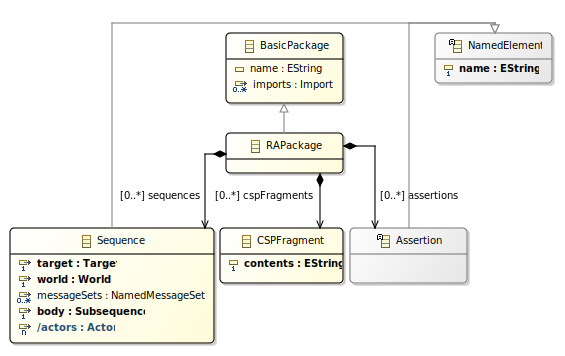
\includegraphics[width=.85\textwidth]{diagrams/Top}
	\caption{Class diagram for the top of the \langname{} metamodel.}
	\label{fig:metamodel-top}
\end{figure}

\Cref{fig:metamodel-top} is the top-level metamodel diagram for \langname.

Each \langname{} script contains an \mrapackage,\footnote{\mrapackage{} stands
for `RoboStar Assertions package'; we use this name because \mrcpackage{} is
already used for RoboChart packages.}
which is a type of RoboStar \mbasicpackage.
Each \mrapackage{} can contain zero or more of each of these types of content:

\begin{itemize}
\item
	\msequencegroup{}
	(\cref{sec:metamodel-sequences}):
	a sequence diagram group;
\item
	\mcspfragment:
	a CSP fragment, currently not bound to a particular process
	\todo{this will change};
\item
	\massertion{}
	(\cref{sec:metamodel-assertions}):
	an assertion, currently over sequence diagrams only
	\todo{more types of assertion will appear};
\end{itemize}

%%% Local Variables:
%%% mode: latex
%%% TeX-master: "../robocert"
%%% End:
